\documentclass[a4paper,preprint]{elsarticle}

% Packages
\usepackage{amsfonts,amsmath,amssymb}
\usepackage{mathtools}
\usepackage{algorithm}
\usepackage{algpseudocode}
\usepackage{cleveref}
\usepackage{enumitem}
\usepackage{todonotes}

% Remove unwanted spaces in lists
\setlist{nosep}

% Theorem-like environments
\newtheorem{theorem}{Theorem}
\newtheorem{lemma}{Lemma}
\newproof{proof}{Proof}

% Custom macros
\newcommand{\htime}{\tau_\mathrm{end}}
\newcommand{\Val}{\mathrm{Val}}
\renewcommand{\vec}[1]{\boldsymbol{#1}}
\DeclareMathOperator{\Ex}{\mathbb{E}}

\begin{document}

\title{Computation of Expected Epidemic End Time}

\author[1]{Alejandro Alarc\'on Gonz\'alez\corref{cor1}}
\ead{alejandroalarcon.gonzalez@uantwerpen.be}
\author[1]{Guillermo A. P\'erez}
\author[1]{Shrisha Rao}
\cortext[cor1]{Corresponding author}
\affiliation[1]{organization={University of Antwerp -- Flanders Make},
 addressline={Middelheimlaan 1},
 postcode={2020},
 city={Antwerp},
 country={Belgium}}

\begin{abstract}
  TBW
\end{abstract}

\begin{keyword}
  Compartment model \sep stochastic epidemic model \sep Markov chain
\end{keyword}

\maketitle

\section{Introduction}
\begin{itemize}
    \item Mention SIR epimiological models are standard
    \item Motivate the use of SIR models in large populations or give examples of SIR variants already being used with large populations.
    
    \textit{We could maybe draw a parallelism with the use of the basic ode governing SIR dynamics in large populations.}
    \item Mention examples of other exact algorithms for SIR models.
    
    \textit{The books of Bailey and Allen discuss the termination time for the simpler Reed-Frost and Greenwood models. They do so by deriving probability generating functions.} 
    \item \dots
\end{itemize}

\section{Markov Chains}
\todo[inline]{G: add some preliminaries}

\section{Compartment Models}
\todo[inline]{G: Introduce S, I, R, N and the intuition}

When an infectious individual makes contact with a susceptible individual, there is some probability per unit of time that such contact will lead to disease transmission. Such probability is denoted by $\beta$, and we take it to be irrespective of the specific susceptible-infectious pair. Furthermore, we define the \textit{force of infection}, denoted by $\Lambda(t)$, as the probability per unit of time for a susceptible individual to become infected at time t. Assuming \textit{uniform mixing} within the population yields the following relation 

\begin{equation}
\label{eq:lawofmassaction}
\Lambda(t)=\beta I(t),
\end{equation}
when $I(t)$ denotes the number of infectious individuals at time $t$. The exposition above can be illustrated by the following continuous-time relation   

\begin{equation}
\label{eq:diffeq}
    \dfrac{dS}{dt}(t)=-\Lambda(t)S(t),
\end{equation}
%
where the probability $\Lambda(t)$ has turned into a growth rate. We note that by discretizising \eqref{eq:diffeq}, we will obtain expectations since the equation itself carries an averaging process that comes from the uniform mixing premise. We start the discretization by fixing $h=1/24$ days as the length of time between two consecutive model evaluations. By integrating \eqref{eq:diffeq} over the time interval $(t,t+h]$, the recurrence relation 

\begin{equation} 
\label{eq:expectedinS}
        S(t+h)=e^{-\int_{t}^{t+h} \Lambda(\tau)d\tau}S(t) 
\end{equation}
%
is deduced. Equation \eqref{eq:expectedinS} gives the expected number of
susceptibles  at time $t+h$, when we assume that there are $S(t)$ susceptibles
at time $t$. We observe in turn that the first factor on the r.h.s of
\eqref{eq:expectedinS} is the probability for a susceptible to escape from
infection during the time interval $(t,t+h]$. Therefore,
$1-\exp(-\int_{t}^{t+h} \Lambda(\tau)d\tau)$ is the probability for a
susceptible to become infected during the time interval $(t,t+h]$. 

The integral 

\begin{equation}
\label{eq:cumulativeforce}
  \int_{t}^{t+h} \Lambda(\tau)d\tau  
\end{equation}


becomes the cumulative force of infection over $(t,t+h]$. By taking the Taylor expansion of \eqref{eq:cumulativeforce} about $t$ and considering expressions \eqref{eq:lawofmassaction}, \eqref{eq:expectedinS} together, the following holds

\begin{align*} 
\label{eq:expectedinS}
        S(t+h)&=e^{-\int_{t}^{t+h} \beta I(\tau)d\tau}S(t)\\
        &=e^{-\beta(\int_{t}^{t}I(\tau)d\tau+hI(t)+\mathcal{O}( h^2))}S(t)\\
        &\approx e^{-h\beta I(t)}S(t),\text{ for $h$ small.}   
\end{align*}

The probability $p_1(t)=1-e^{-h\beta I(t)}$ will now be regarded as the success probability  for the Bernoulli trial corresponding to an interaction between an infectious and a susceptible individual, and the interaction occurs within $(t,t+h]$\footnote{Abrams et al. \cite{abrams21} take the value $h=1/24$, explain why.}. By recalling the assumption of uniform mixing, the discussion of this section can be summarized with the following relation

\begin{equation}
\label{eq:CBI}
\vec{I}_{t+h}^{new}\sim B(\vec{S}_t, p_1(t)=1-\exp(-h\beta \vec{I}_t)).
\end{equation}

To finish this modelling part, the infectious period $\Delta(t)$ is assumed to be exponentially distributed with parameter $\gamma \in \mathbb{R}$, irrespectively of the individual. Accordingly, the cumulative density function $p_2(t)=1-\exp(-t\gamma)$ will represent the probability for an infectious individual to have recovered by time $t>0$. The corresponding number of newly recovered individuals within $(t,t+h]$ is then given by

\begin{equation} 
    \label{eq:CBR}
    \vec{R}_{t+h}^{new}\sim B(\vec{I}_t, p_2=1-\exp(-h\gamma)).
\end{equation}

The expressions \eqref{eq:CBI} and \eqref{eq:CBR} yield the \textit{chain-binomial model}, to be introduced in the next section.


\begin{figure}[t]
  \centering
  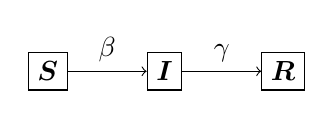
\begin{tikzpicture}
    \node[rectangle,draw](s){$\vec{S}$};
    \node[rectangle,draw,right= of s](i){$\vec{I}$};
    \node[rectangle,draw,right= of i](r){$\vec{R}$};
    \path[->,auto]
      (s) edge node{$\beta$} (i)
      (i) edge node{$\gamma$} (r);
  \end{tikzpicture}
\caption{Overview of the flow of individuals in the compartmental model:
Following a disease infection, susceptible individuals ($\vec{S}$) move to an
infectious state ($\vec{I}$) in which they can infect others. Such infectious
individuals will recover over time.}
\label{fig:flow_diagram}
\end{figure}

\section{Discrete-Time Stochastic Epidemic Model}

Our \textit{chain-binomial model}, is now introduced based on the previously described infection and recovery events. The model takes the form of a discrete-time stochastic process 

\begin{equation}
\label{eq:SIRmodel}
  \{X_{t} \mbox{, }t=0,h,2h,\ldots\}=\{(\vec{S}_{t}, \vec{I}_{t}, \vec{R}_{t}) \mbox{, }t=0,h,2h,\ldots\},  
\end{equation}

where the sequence of random variables $\{(\vec{S}_{t}, \vec{I}_{t}, \vec{R}_{t})\}$ is defined recursively as follows
\begin{align}
\label{eq:difference_equations}
    \vec{S}_{t+h} = {} & \vec{S}_{t} - \vec{I}_{t+h}^{new}, \\
    \vec{I}_{t+h} = {} & \vec{I}_{t} + \vec{I}_{t+h}^{new} - \vec{R}_{t+h}^{new}, \\
    \vec{R}_{t+h} = {} & \vec{R}_{t} + \vec{R}_{t+h}^{new}, 
\label{eq:difference_equations_again}
\end{align}
%
and $\vec{I}_{t+h}^{new}$ and $\vec{R}_{t+h}^{new}$ are obtained from \eqref{eq:CBI} and \eqref{eq:CBR}, respectively. Observe that $\{X_{t}\}$ satisfies the \textit{conservative} condition $\vec{S}_t+\vec{I}_t+\vec{R}_t=N$, for $t=0,h,2h,\ldots$ Furthermore, $\{X_{t}\}$ satisfies the \textit{memory-less} property, i.e., the state of the system at time $t+h$ only depends on the state of the system at time $t$, and thus $\{X_{t}\}$ is a discrete-time Markov Chain $\mathcal{C}$. The terms for the corresponding
probability transition matrix $P$ will now be derived. It will be convenient to write $P(\vec{m},\vec{n})$ to denote the entry of $P$ corresponding to the probability of transitioning from state $\vec{m}$ to $\vec{n}$.



First note that the Markov chain \eqref{eq:SIRmodel} can be simplified to $\{(\vec{S}_{t}, \vec{R}_{t}) \mbox{, }t=0,h,2h,\ldots\}$, since $\vec{I}_{t}$ can be (deterministically) obtained as $\vec{I}_{t}=N-\vec{S}_{t}-\vec{R}_{t}$. In the following, we will construct the joint probability mass function of $\vec{S}_{t}$ and $\vec{R}_{t}$. Taking \eqref{eq:difference_equations} and \eqref{eq:CBI} together, the probability mass function  $p_S$ corresponding to $\vec{S}_{t}$ is obtained as follows

\begin{equation}
\begin{split}
\label{eq:Spmf}
p_S(n_1)=&P(\vec{S}_{t+h}=n_1)\\
={} & P(\vec{S}_{t}-\vec{I}_{t+h}^{new}=n_1\mid \vec{S}_{t}=m_1,\vec{I}_{t}=m_2) \\
={} & P(\vec{I}_{t+h}^{new}=m_1-n_1\mid \vec{I}_{t}=m_2) \\
={} & {\binom{m_1}{m_1-n_1}}(1-p_1(t))^{n_1}p_1(t)^{m_1-n_1},       
\end{split}
\end{equation}
%
for $n_1=0,1,\ldots,m_1$. (Here, we adopt the convention that $0^0 = 1$ for $p_S(m_1)$ to be $1$ when $m_2 = 0$.) In turn, taking \eqref{eq:difference_equations_again} and \eqref{eq:CBR} together, the probability mass function  $p_R$ corresponding to $\vec{R}_{t}$ is obtained as follows 

\begin{equation}
\begin{split}
\label{eq:Rpmf} 
p_R(n_3)=&P(\vec{R}_{t+h}=n_3 \mid \vec{I}_{t}=m_2 \mbox{, } \vec{R}_{t}=m_3)\\    
=&P(\vec{R}_{t} + \vec{R}_{t+h}^{new}=n_3 \mid \vec{I}_{t}=m_2 \mbox{, } \vec{R}_{t}=m_3) \\
=&P(\vec{R}_{t+h}^{new}=n_3-m_3 \mid \vec{I}_{t}=m_2 \mbox{, } \vec{R}_{t}=m_3) \\
=& {\binom{m_2}{n_3-m_3}}(1-\exp(-h\gamma))^{n_3-m_3}\exp(-h\gamma)^{m_2-n_3+m_3},      
\end{split}
\end{equation}
for $n_3-m_3=0,1,\ldots,m_2$. Observe from \eqref{eq:Spmf} and \eqref{eq:Rpmf} that $\vec{S}_{t}$ and $\vec{R}_{t}$ are independent\footnote{Recall that if $X$ and $Y$ are independent then $P(X= x,Y= y)=P(X= x)P(Y= y)=p_{X}(x)p_{Y}(y)$ for $x,y$ in the sample space.}, and thus, the joint probability mass function $p_{SR}$ of $\vec{S}_{t}$ and $\vec{R}_{t}$ is given by
%
\begin{equation}
\label{eq:jpmf} 
p_{SR}(n_1,n_3)=p_S(n_1)p_R(n_3).    
\end{equation}
%
Note that the probability transition matrix $P$ of the Markov chains $\{\vec{S}_{t},\vec{R}_{t}\}$ and $\{\vec{S}_{t},\vec{I}_{t}, \vec{R}_{t}\}$ is given by $p_{SR}$. That is,  
for any $\vec{n}=(n_1,N-n_1-n_3,n_3)$ and $\vec{m}=(m_1,m_2,m_3)$ such that $n_1=0,1,\ldots,m_1$ and $n_3-m_3=0,1,\ldots,m_2$ we have the following
\begin{equation}
\label{eqn:finalform}
P((\vec{S}_{t+h}, \vec{I}_{t+h}, \vec{R}_{t+h})=\vec{n}\mid (\vec{S}_{t}, \vec{I}_{t}, \vec{R}_{t})=\vec{m})
=p_{SR}(n_1,n_3)>0.
\end{equation}
%
On the other hand, if the inequalities  $0\leq n_1\leq m_1$ and $0\leq m_3 \leq n_3 \leq m_3+m_2$ are not satisfied, then $P(\vec{m},\vec{n})=0$. 

To conclude this section we state the following property which follows immediately from the above definition of the transition matrix $P$.
\begin{lemma}\label{lem:succ}
    Let $\vec{m},\vec{n}$ be states. Then, $P(\vec{m},\vec{n}) \neq 0$ if
    and only if $n_1 \leq m_1$ and $m_3 \leq n_3 \leq m_2 + m_3$.
\end{lemma}

%In general, for a finite family of events $\{A_i\}$ and $\mathbb{P}$ a probability function, the following relation holds

%\begin{equation}
%    \label{eq:intersection_probability}   
%    \mathbb{P}\left( \bigcap_{i=1}^{n}A_{i}\right)=\mathbb{P}\left(A_n\mid \bigcap_{i=1}^{n-1}A_{i}\right)\mathbb{P}\left(A_{n-1}\mid \bigcap_{i=1}^{n-2}A_{i}\right)\ldots \mathbb{P}\left(A_2\mid A_{1}\right)\mathbb{P}\left(A_{1}\right). 
%\end{equation}

%\medskip
%Observe that the state space $\mathcal{A}$ for the process $\{X_t\}$ is composed of the vectors $(a,b,c)\in \mathbb{N}^3$ such that $a+b+c=N$. Let $\vec{m}\in \mathcal{A}$, $n_1, n_2\in \mathbb{N}$, with $n_1+n_2\leq N$, and the family of events $\{A_i\}_{i=1}^{3}$ be defined as follows


%\begin{equation*}
%\begin{split}
%&A_1:=S_{t+h}=n_1 \mbox{, } I_{t+h} \in \{0,1,\ldots, N-n_1\} \mid X_t=\vec{m},\\
%&\mbox{ and conservation holds,}\\%need to mention that the other variables are free²
%&A_2:=I_{t+h}=n_2 \mbox{, } S_{t+h} \in \{0,1,\ldots, N-n_2\} \mid X_t=\vec{m},\\
%&\mbox{ and conservation holds,}\\ 
%&A_3:=R_{t+h}=n_3 = N-n_1-n_2 \mbox{, } S_{t+h} \in \{0,1,\ldots, n_1+n_2\} \mid X_t=\vec{m}. \\
%&\mbox{ and conservation holds,}
%\end{split}
%\end{equation*}

%Due to the conservation property these events are fully defined, even though only two coordinates are explicitly given. To illustrate this, take $S_{t+h}=n_1$ and $I_{t+h}=n_2$, then $R_{t+h}$ must be equal to $N-n_1-n_2$ in order for $(S_{t+h},I_{t+h},R_{t+h})$ to be in $\Omega$ . Note that this example leads to the expression $\mathbb{P}\left(A_3\mid A_{1}\cap A_{2}\right)=\mathbb{P}\left(A_{1}\cap A_{2}\right)$.%  Furthermore, if $A_4:=R_{t+h}=n_4$ s.t.  $n_4\neq N-n_1-n_2$, then $\mathbb{P}\left(A_4\mid A_{1}\cap A_{2}\right)=0$, since $n_1+n_2+n_4\neq N$. 

%By construction of $A_1,A_2,A_3$, observe that the following relation holds true
%\[P({\vec{m},\vec{n}})=\mathbb{P}\left( \bigcap_{i=1}^{3}A_{i}\right),\]
%where $\mathbb{P}=P_{\mathcal{C}}$ is the probabilistic function induced by our Markov chain. Therefore, it is enough to compute each of the terms on the r.h.s. of equation \eqref{eq:intersection_probability} in order the get $P({\vec{m},\vec{n}})$. This defines the procedure that follows next.





\section{The Expected Epidemic End Time}
In this section we are interested in computing the expected \emph{hitting
time} to the set of states where no infectious individuals remain. That is, we
want to compute the expected time to the end of the epidemic. Formally, we
write $\htime$ for the random variable whose value is defined as follows.
\[
    \htime \coloneqq \inf\{t \in \mathbb{N} \mid X_t = \vec{m}, m_2 = 0\}
\]
%
Let us write $\Ex^{\vec{m}}[\htime]$ to denote the expected value of $\htime$ with respect to the probability function induced by our Markov
chain with $\vec{m}$ as initial state. From the well-known linear recurrence
satisfied by hitting times~\cite{norris98} and \Cref{lem:succ}, we get the
following.
\begin{lemma}\label{lem:belleq}
    For all states $\vec{m}$, we have that $\Ex^{\vec{m}}[ \htime ]$ is:
    \[
        \begin{cases}
            0 & \text{if } m_2 = 0,\\
            1 + \sum_{n_1 = 0}^{m_1} \sum_{n_3 = m_3}^{m_2+m_3}
            P(\vec{m},\vec{n}) \Ex^{\vec{n}}[\htime] & \text{otherwise,}
        \end{cases}
    \]
    where $\vec{n} = (n_1,N-n_1-n_3,n_3)$.
\end{lemma}

Note that the above lemma gives us an algorithm to compute $\Ex^{\vec{m}}[\htime]$ from any given $\vec{m}$.

\subsection{A simple algorithm}
\Cref{alg:simple} exploits the lack of cycles in the Markov chain
to apply the equalities from \Cref{lem:belleq}
in order to compute the expected hitting times from all states. Notice that, by
conservation of population, two for-loops suffice to go through all source and
target states. That is, in line \ref{loc:n} no further for-loop is needed
since there is a unique value of $n_2$ that makes $(n_1,n_2,n_3)$ a valid
state. Further note that in line \ref{loc:M} we cycle through all values of
$m_1 + m_2$ which is why the following for-loop runs until $M$. Then, similar
to the case of $\vec{n}$, no further for-loop is needed since there is a
unique value of $m_3$ such that $(M-m_2,m_2,m_3)$ is a valid state.

The next property, which follows directly from \Cref{lem:succ}, will be useful
in our analysis of \Cref{alg:simple}.
\begin{lemma}\label{lem:order}
  Let $\vec{m},\vec{n}$ be states. If $P(\vec{m},\vec{n}) > 0$ then:
  \begin{itemize}
    \item either $\vec{m} = \vec{n}$ or
    \item $m_1 \geq n_1$, $m_1 + m_2 \geq n_1 + n_2$, and one of the latter
      two is strict.
  \end{itemize}
\end{lemma}

\begin{algorithm}[t]
    \caption{A simple algorithm to compute $\Ex^{\vec{m}}[\htime]$ from all $\vec{m}$}
    \label{alg:simple}
    \begin{algorithmic}[1]
      \For{$m_1=1,\dots,N$} \Comment{Initialize value of target states}
          \State $\Val(\vec{m}) \gets 0$, with $\vec{m} = (m_1,0,N-m_1)$
      \EndFor \label{loc:endinit}
      \For{$M = 1, \dots, N$} \Comment{Compute value of other states} \label{loc:M}
          \For{$m_2 = 1, \dots, M$}
              \State $\vec{m} \gets (M - m_2,m_2,N-M)$ \label{loc:m}
              \State $\Val(\vec{m}) \gets 1$ \label{loc:initval}
              \For{$n_3 = m_3, \dots, m_2+m_3$}
                  \For{$n_1 = 0, \dots, m_1$} \label{loc:inner}
                     \State $\vec{n} = (n_1,N-n_1-n_3,n_3)$ \label{loc:n}
                      \If{$\vec{m} \neq \vec{n}$} \Comment{Ignore self-loops}
                          \State $\Val(\vec{m}) \gets \Val(\vec{m}) +
                          P(\vec{m},\vec{n})\Val(\vec{n})$ \label{loc:rec}
                      \EndIf
                  \EndFor \label{loc:endinner}
              \EndFor \label{loc:endloopsm}
              \State $\Val(\vec{m}) \gets \Val(\vec{m}) /
              (1-P(\vec{m},\vec{m}))$ \Comment{Add self-loops}
              \label{loc:norm}
          \EndFor
      \EndFor
    \end{algorithmic}
\end{algorithm}

Note that \Cref{alg:simple} clearly terminates. Further observe that the
algorithm has $4$ nested for-loops, each ranging over at most $N$ values
each. Since $P(\vec{m},\vec{n})$ can be calculated using $O(N)$ elementary
operations\footnote{We take binary addition and multiplication to be
elementary operations. Hence, while exponentiation can be realized using a
logarithmic number of such operations via iterated squaring, we are not
aware of an algorithm to compute factorials using a sub-linear number of
multiplications.}
using \eqref{eqn:finalform}, we get the following more
precise statement.
\begin{theorem}[Complexity]
  The worst-case time complexity of \Cref{alg:simple} is
  $O(N^5)$.
\end{theorem}

Regarding the values that the algorithm computes, we can prove that they are
indeed the required expected hitting times.
\begin{theorem}[Correctness]
  Let $\Val(\cdot)$ be as computed by \Cref{alg:simple}.  Then, $\Val(\vec{m})
  = \Ex^{\vec{m}}[\htime]$ for all states $\vec{m}$.
\end{theorem}
\begin{proof}
  First, note that \Cref{lem:order} guarantees $\Val(\vec{n})$ has already
  been computed when used in line \ref{loc:rec}. Second, we can focus on
  $\Val(\vec{m})$ such that $m_2 > 0$ since for the remaining $\vec{m}$, the
  claim holds already after the initialization ends in line \ref{loc:endinit}.

  Now, for an arbitrary $\vec{m}$ as computed in line \ref{loc:m} let
  $\Val_1(\vec{m})$ denote the value of $\Val(\vec{m})$ after line
  \ref{loc:initval} is executed; $\Val_2(\vec{m})$ its value after line
  \ref{loc:endloopsm} is executed; and $\Val_3(\vec{m})$ its value after line
  \ref{loc:norm}. We will argue that $\Val_3(\vec{m}) =
  \Ex^{\vec{m}}[\htime]$, which will conclude the argument because
  $\Val(\vec{m})$ is not updated afterwards. Note that the following hold.
  \begin{align*}
    \Val_2(\vec{m}) &{} = \Val_1(\vec{m}) + \sum_{n_1 = 0}^{m_1} \sum_{n_3 = m_3}^{m_2+m_3}
            P(\vec{m},\vec{n}) \Ex^{\vec{n}}[\htime] -
            P(\vec{m},\vec{m})\Ex^{\vec{m}}[\htime]\\
                    &{} = 1 + \sum_{n_1 = 0}^{m_1} \sum_{n_3 = m_3}^{m_2+m_3}
            P(\vec{m},\vec{n}) \Ex^{\vec{n}}[\htime] -
            P(\vec{m},\vec{m})\Ex^{\vec{m}}[\htime]\\
                    &{} = \Ex^{\vec{m}}[\htime] -
            P(\vec{m},\vec{m})\Ex^{\vec{m}}[\htime]\\
                    &{} = \Ex^{\vec{m}}[\htime](1 - P(\vec{m},\vec{m}))
  \end{align*}
  Finally, since $\Val_3(\vec{m}) = \Val_2(\vec{m})/(1-P(\vec{m},\vec{m}))$,
  we get that $\Val_3(\vec{m}) = \Ex^{\vec{m}}[\htime]$.\qed
\end{proof}

The question is now: can one do better? In the next section we give a positive
answer to this question by improving on our algorithm using dynamic
programming to efficiently pre-compute the values $P(\vec{m},\vec{n})$ for all $\vec{m}$ and $\vec{n}$.

\subsection{A more efficient algorithm}
Recall \eqref{eqn:finalform} gives us that for all
states $\vec{m} \neq \vec{n}$ such that $n_1 \leq m_1$ and $m_3 \leq n_3 \leq
m_2 + m_3$ the probability $P(\vec{m},\vec{n})$ of transitioning from $\vec{m}$ to $\vec{n}$ is as
follows.
\begin{align}
  & \binom{m_1}{m_1-n_1}\exp(-h\beta m_2)^{n_1}
  (1-\exp(-h\beta m_2))^{m_1-n_1} \label{eqn:final-si}\\
  {}\times{} & \binom{m_2}{n_3-m_3}(1-\exp(-h\gamma))^{n_3-m_3}\exp(-h\gamma)^{m_2-n_3+m_3} \label{eqn:final-ir}
\end{align}
%
The crux of our improvement on \Cref{alg:simple} is the following recurrence.
\begin{lemma}\label{lem:recrel}
  Let $\vec{m},\vec{n}$ be states such that $n_1 < m_1$ and $m_3 < n_3 \leq m_2 + m_3$. Then, \(
    P(\vec{m},\vec{n}) = \alpha(\vec{m},\vec{n}) P(m_1-1,m_2,m_3+1,\vec{n}),
  \) where:
  \[
      \alpha(\vec{m},\vec{n}) \coloneqq 
      \frac{m_1(m_2-n_3+m_3+1)(1-\exp(-h\gamma))(1-\exp(-h\beta m_2))}{(n_3-m_3)(m_1-n_1)\exp(-h\gamma)}.
  \]
\end{lemma}
\begin{proof}
  Note that $P(\vec{m},\vec{n}), P(m_1-1,m_2,m_3+1,\vec{n})> 0$ by
  \Cref{lem:succ} and our assumptions.
  We first consider the binomial coefficients of \eqref{eqn:final-si} and \eqref{eqn:final-ir}.
  \begin{align*}
    & \binom{m_1}{m_1-n_1} \binom{m_2}{n_3-m_3}\\
    {}={} & \frac{m_1(m_2-n_3+m_3+1)}{(n_3-m_3)(m_1-n_1)} \binom{m_1-1}{m_1-1-n_1}
    \binom{m_2}{n_3-(m_3+1)}
  \end{align*}
  Importantly, since we have assumed that $m_3 < n_3$ and $n_1 < m_1$, the denominator of the fraction above is not $0$.
  On the other hand, for the terms involving ``probabilities'' --- that is, exponential terms --- we observe that the following is true for \eqref{eqn:final-si}.
  \begin{align*}
  & \exp(-h\beta m_2)^{n_1}
  (1-\exp(-h\beta m_2))^{m_1-n_1}\\ {}={} &(1-\exp(-h\beta m_2)) \exp(-h\beta m_2)^{n_1}
  (1-\exp(-h\beta m_2))^{m_1-1-n_1}
  \end{align*}
  %
  Similarly, for the probabilities in \eqref{eqn:final-ir} we note the following.
  %
  \begin{align*}
    & (1-\exp(-h\gamma))^{n_3-m_3}\exp(-h\gamma)^{m_2-n_3+m_3}\\
    {}={} & \frac{1-\exp(-h\gamma)}{\exp(-h\gamma)} (1-\exp(-h\gamma))^{n_3-(m_3+1)}\exp(-h\gamma)^{m_2-n_3+m_3+1}
  \end{align*}
  Indeed, $\alpha(\vec{m},\vec{n})$ is exactly the product of the coefficients on the right-hand sides of the above equalities. This concludes the proof as the product of the left-hand sides is exactly $P(\vec{m},\vec{n})$ and that of the right-hand sides (after factoring out $\alpha$) is $P(m_1-1,m_2,m_3+1,\vec{n}$).\qed
\end{proof}

Based on \Cref{lem:recrel}, we propose \Cref{alg:probs} to compute $P(\vec{m},\vec{n})$ for all $\vec{m}$ and $\vec{n}$. The recurrence relation allows us to compute new transition probabilities based on previously computed ones in a manner reminiscent of how Pascal's rule is used to construct Pascal's triangle.

\begin{algorithm}[t]
    \caption{An efficient algorithm to compute $P(\vec{m},\vec{n})$ for all $\vec{m}$ and $\vec{n}$}
    \label{alg:probs}
    \begin{algorithmic}[1]
        \For{$m_1 = 0, \dots,
        N$}
            \State $X(\vec{m},\vec{m}) = 1$, with $\vec{m} = (m_1,0,N-m_1)$
        \EndFor
        \For{$M = 1, \dots, N$}
          \For{$m_2 = 1, \dots, M$}
              \State $\vec{m} \gets (M - m_2,m_2,N-M)$
              \For{$n_3 = m_3, \dots,m_2+m_3$} \Comment{Fix $n_1=m_1$}
                \State $X(\vec{m},\vec{n}) \gets P(\vec{m},\vec{n})$, with $\vec{n}=(m_1,N-m_1-n_3,n_3)$\label{loc:fixn1}
              \EndFor
              \For{$n_1 = 0, \dots,m_1$} \Comment{Fix $n_3=m_3$}
                \State $X(\vec{m},\vec{n}) \gets P(\vec{m},\vec{n})$, with $\vec{n}=(n_1,N-n_1-m_3,m_3)$\label{loc:fixn3}
              \EndFor
              \For{$n_3 = m_3+1, \dots, m_2+m_3$}\label{loc:reccomp-start}
                  \For{$n_1 = 0, \dots, m_1-1$}
                     \State $\vec{n} \gets (n_1,N-n_1-n_3,n_3)$
                     \State $\vec{m'} \gets (m_1-1,m_2,m_3+1)$
                     \State $X(\vec{m},\vec{n}) \gets \alpha(\vec{m},\vec{n})X(\vec{m'},\vec{n})$
                  \EndFor
              \EndFor\label{loc:reccomp-end}
          \EndFor
      \EndFor
    \end{algorithmic}
\end{algorithm}

As with \Cref{alg:simple}, we observe that \Cref{alg:probs} clearly terminates because all for-loops are bounded and there are no jump statements in the code. Regarding the time complexity of \Cref{alg:probs}, however, we now only ever nest at most $4$ for-loops and $P(\vec{m},\vec{n})$ is never used (i.e. computed) in an innermost loop.
\begin{theorem}[Complexity]
    The worst-case time complexity of \Cref{alg:probs} is $O(N^4)$.
\end{theorem}

For correctness, we have the following statement.
\begin{theorem}[Correctess]
    Let $X(\cdot)$ be as computed by \Cref{alg:probs}. Then, $X(\vec{m}, \vec{n}) = P(\vec{m},\vec{n})$ for all pairs of states $\vec{m}, \vec{n}$ such that $n_1 \leq m_1$ and $m_3 \leq n_3 \leq m_2 + m_3$.
\end{theorem}
\begin{proof}
    First, one needs to take care that the previous transition probabilities must be defined before they are being used. Note that this is only relevant in lines \ref{loc:reccomp-start}--\ref{loc:reccomp-end}. It thus follows from the order in which the states $\vec{m}$ are traversed that $X(\vec{m'},\vec{n})$ has already been computed in a previous iteration.
    
    Now, it is easy to see that $X(\vec{m},\vec{n}) = P(\vec{m},\vec{n})$ if either $m_1 = n_1$ or $m_3 = n_3$ since lines \ref{loc:fixn1} and \ref{loc:fixn3} literally assign the right-hand side to the left-hand side of the equality. If neither equality holds, then $X(\vec{m},\vec{n})$ is computed in the loop \ref{loc:reccomp-start}--\ref{loc:reccomp-end} and $X(\vec{m},\vec{n}) = P(\vec{m},\vec{n})$ by \Cref{lem:recrel}.\qed
\end{proof}

Together with the theorems regarding \Cref{alg:simple}, the above imply the following.
\begin{theorem}
    \Cref{alg:simple}, when pre-computing $P(\vec{m},\vec{n})$ using \Cref{alg:probs}, computes $\Ex^{\vec{m}}[\htime]$ for all states $\vec{m}$ in time $O(N^4)$.
\end{theorem}

\section{Relations between chain binomial and ode}

Observe that 
$\mathbb{E}[I_{t+h}^{new}]=S_t p_1(t)$ and consider the system
\begin{align}
\label{eq:difference_equations}
    \vec{S}_{t+h} = {} & \vec{S}_{t} - \mathbb{E}[\vec{I}_{t+h}^{new}], \\
    \vec{I}_{t+h} = {} & \vec{I}_{t} + \mathbb{E}[\vec{I}_{t+h}^{new}] - \mathbb{E}[\vec{R}_{t+h}^{new}], \\
    \vec{R}_{t+h} = {} & \vec{R}_{t} + \mathbb{E}[\vec{R}_{t+h}^{new}]. 
    \label{eq:difference_equationsnext}
\end{align}


Working out \eqref{eq:difference_equations} with the identity $\exp(x)=\sum_{k=0}^{\infty}\left(\dfrac{x^k}{k!}\right)$ yields the following

\begin{equation*}
    \begin{split}
    \vec{S}_{t+h}-\vec{S}_{t} = {} & -\mathbb{E}[\vec{I}_{t+h}^{new}]\\
    ={}&-p_1(t)\vec{S}_{t}\\
    ={}&(\exp(-h\beta I_t))-1)\vec{S}_{t}\\
    ={}&\sum_{k=1}^{\infty}\dfrac{(-h\beta I_t)^k}{k!}\vec{S}_{t}\\
    ={}&\sum_{k=2}^{\infty}\dfrac{(-h\beta I_t)^k}{k!}\vec{S}_{t}-h\beta I_t S_t,
    \end{split}\end{equation*}

and thus
\begin{equation}
\label{eq:cauchy}
\dfrac{\vec{S}_{t+h}-\vec{S}_{t}}{h}=\sum_{k=2}\dfrac{(-h)^{k-1}(\beta I_t)^{k}}{k!}\vec{S}_{t}-\beta I_t S_t.
\end{equation}

By taking the limit $h\rightarrow{0}$ in \eqref{eq:cauchy}, the relation $dS/dt =  -\beta SI$ is retrieved. We can conclude that the system \eqref{eq:difference_equations}-\eqref{eq:difference_equationsnext} solves the deterministic $SIR$ when $h\rightarrow{0}$. 

\section*{Acknowledgments}
We would like to thank Kasper Engelen for proof-reading the article and the code of our implementation.
Financial support for this work was provided by the Flemish inter-university (iBOF) ``DESCARTES'' project.



\bibliographystyle{elsarticle-num}
\bibliography{refs}

\end{document}
